\documentclass[12pt,a4paper]{article}
\usepackage[utf8]{inputenc}
\usepackage[brazil]{babel}
\usepackage{graphicx}
\usepackage{hyperref}
\usepackage{abnt-alf}
\usepackage[top=3cm,bottom=2cm,left=3cm,right=2cm]{geometry}
\usepackage{indentfirst}

\begin{document}

% CAPA
\pagestyle{empty}
\begin{center}
\large  \textbf{UNIVERSIDADE PRESBITERIANA MACKENZIE}
\large  \textbf{PROGRAMA DE PÓS-GRADUAÇÃO EM}\\
\large  \textbf{ENGENHARIA ELÉTRICA E COMPUTAÇÃO}\\
\vskip 2.0cm
\textbf{\large Afonso Cesar Lelis Brandão}\\
\vskip 4.0cm
\setlength{\baselineskip}{1.5\baselineskip}
\textbf{\large Modelo de Gêmeo Digital de Processos e Sistemas para Avaliações em Project Based Learning}\\
\vskip 4.5cm
\end{center}
\hfill{\vbox{\hsize=8.5cm\noindent\strut
Projeto de Pesquisa apresentado ao Programa\break
de Pós-Graduação em Engenharia Elétrica e\break
Computação da Universidade Presbiteriana\break
Mackenzie como parte dos requisitos para\break
qualificação no programa de doutorado.}\\
\strut}
\vskip 3.0cm
\textbf{\normalsize Orientador: Dr. Ismar Frango Silveira}\\
\vskip 2.0cm
\begin{center}
São Paulo, 2025\\
\end{center}

% RESUMO
\newpage
\thispagestyle{plain}
\pagenumbering{roman}
\begin{center}
\large
\textbf{RESUMO}
\end{center}
\renewcommand{\baselinestretch}{0.6666666}
Em criação.
\\[0.5cm]
\begin{flushleft}
{\bf Palavras-chave:} {\it palavra 1, 2, 3...}
\end{flushleft}

% SUMÁRIO
\newpage
\thispagestyle{empty}
\tableofcontents

% DESENVOLVIMENTO
\newpage
\pagestyle{plain}
\pagenumbering{arabic}
\renewcommand{\baselinestretch}{1.5}
\normalsize
\section{INTRODUÇÃO}

A Aprendizagem Baseada em Projetos (Project-Based Learning - PBL) tem se consolidado como uma metodologia educacional que apresenta resultados documentados no desenvolvimento de competências técnicas e transversais em cursos de engenharia, com foco específico na integração entre teoria e prática através de projetos autênticos \cite{zhang2023, lavado2024, guo2020}. Esta abordagem pedagógica, centrada na resolução de problemas reais e complexos, promove o aprendizado experiencial através da execução de projetos práticos que integram conhecimentos teóricos e aplicações práticas. O desenvolvimento de métodos eficazes para avaliação da aprendizagem neste contexto requer a adoção de critérios estruturados que contemplem múltiplas dimensões do processo educacional, incluindo aspectos de utilidade, viabilidade, propriedade e precisão dos instrumentos de avaliação.

No contexto contemporâneo, os Gêmeos Digitais (Digital Twins) emergem como uma tecnologia com potencial transformador que pode oferecer representações virtuais dinâmicas e interativas de sistemas, processos ou entidades, não necessariamente limitados ao domínio físico \cite{grieves2014, tao2018}. Diferentemente de simulações estáticas tradicionais, os gêmeos digitais mantêm sincronização contínua com seus equivalentes reais, permitindo monitoramento em tempo real, análise preditiva e otimização de processos \cite{silveira2024panorama}. Esta tecnologia tem encontrado aplicações promissoras na educação em engenharia, especialmente quando integrada à metodologia PBL, conforme indicado em estudos recentes que apresentam casos práticos de desenvolvimento de protótipos físicos e virtuais por estudantes de engenharia \cite{bachmann2023}.

A taxonomia de gêmeos digitais estabelece quatro categorias principais: gêmeos de componente, que representam elementos individuais; gêmeos de produto/ativo, que modelam sistemas completos; gêmeos de sistema, que abrangem múltiplos ativos interconectados; e gêmeos de processo, que simulam fluxos de trabalho e procedimentos operacionais \cite{barricelli2019}. Silveira \cite{silveira2024panorama} complementa esta classificação destacando que, no contexto educacional, os gêmeos digitais de processo são particularmente adequados para modelagem de metodologias pedagógicas ativas, diferenciando-se de simulações estáticas por sua capacidade de atualização contínua e interatividade em tempo real. Para o contexto educacional de PBL, esta categoria apresenta relevância específica, pois possibilita a modelagem e avaliação sistemática dos processos de aprendizagem, incluindo a estrutura pedagógica, o comportamento dos estudantes durante a execução dos projetos e a assimilação progressiva dos conceitos do meta-projeto. A aplicação efetiva desta categoria de gêmeo digital requer a definição de métricas e indicadores que atendam aos critérios de confiabilidade, validade, usabilidade, objetividade e normalização estabelecidos para instrumentos de avaliação educacional.

No âmbito da engenharia de software, a aplicação de visões arquiteturais tradicionais como estrutural, comportamental e de processo pode ser adaptada para caracterizar meta-projetos PBL. A visão estrutural define a organização dos componentes do projeto, incluindo recursos, ferramentas e artefatos. A visão comportamental modela as interações dinâmicas entre estudantes, orientadores e sistema durante a execução do projeto. A visão de processo mapeia os fluxos de atividades, marcos de entrega e critérios de avaliação. Esta abordagem arquitetural permite uma compreensão sistemática dos elementos que compõem um projeto PBL e suas inter-relações, fundamentando a criação de instrumentos de avaliação que contemplem a responsividade às necessidades dos stakeholders, a justificação de conclusões baseadas em evidências e a utilização efetiva de recursos.

Apesar dos avanços na aplicação de gêmeos digitais em contextos educacionais, observa-se uma lacuna significativa na literatura quanto à aplicação específica desta tecnologia para avaliação sistemática de projetos em PBL na área de engenharia de software. As iniciativas existentes concentram-se predominantemente na criação de protótipos físicos e virtuais \cite{bachmann2023}, não abordando adequadamente a avaliação contínua e multidimensional dos processos de aprendizagem. Esta lacuna torna-se particularmente relevante quando se considera a necessidade de implementar sistemas de avaliação que atendam aos padrões de excelência educacional, contemplando critérios de efetividade, eficiência, impacto e sustentabilidade no contexto de programas de engenharia.

\subsection{Objetivo Geral}

Desenvolver um modelo de gêmeo digital de processos e sistemas para avaliação contínua e multidimensional de projetos em Project-Based Learning na área de engenharia de software, integrando as visões arquiteturais estrutural, comportamental e de processo para proporcionar feedback em tempo real sobre a assimilação de conceitos, evolução do aprendizado e qualidade dos artefatos produzidos.

\subsection{Objetivos Específicos}

\begin{itemize}
\item Conceituar um modelo que integre gêmeos digitais de processo com metodologias PBL para engenharia de software;
\item Definir métricas e indicadores de desempenho para avaliação multidimensional de projetos PBL utilizando as três visões arquiteturais (estrutural, comportamental e de processo);
\item Modelar a arquitetura do gêmeo digital contemplando a captura, processamento e análise de dados provenientes da execução de projetos PBL;
\item Implementar um protótipo funcional do modelo proposto integrando ferramentas de desenvolvimento, controle de versão e plataformas de colaboração;
\item Validar o modelo através de estudos de caso em disciplinas de engenharia de software, comparando os resultados com métodos tradicionais de avaliação;
\item Estabelecer diretrizes para implantação e escalabilidade do modelo em diferentes contextos educacionais.
\end{itemize}

\subsection{Hipótese}

\subsubsection{Hipótese Principal}

A implementação de um modelo de gêmeo digital de processos e sistemas, integrado às visões arquiteturais estrutural, comportamental e de processo, proporciona avaliação mais eficaz, objetiva e contínua de projetos em Project-Based Learning na área de engenharia de software quando comparado aos métodos tradicionais de avaliação pontual, resultando em:

\begin{itemize}
\item \textbf{Maior precisão na identificação de dificuldades de aprendizagem}: O monitoramento contínuo permite detectar padrões de comportamento e desempenho que indicam obstáculos no processo de assimilação de conceitos antes que se manifestem como deficiências nos produtos finais;

\item \textbf{Redução da subjetividade na avaliação}: A coleta automatizada de métricas objetivas sobre o processo de desenvolvimento (commits, refatorações, testes, colaboração) complementa e fundamenta a avaliação docente com dados quantitativos e qualitativos consistentes;

\item \textbf{Melhoria na qualidade do feedback pedagógico}: A disponibilidade de dados em tempo real sobre múltiplas dimensões do processo de aprendizagem permite intervenções pedagógicas mais oportunas, específicas e personalizadas;

\item \textbf{Aumento do engajamento e autorregulação dos estudantes}: A visibilidade contínua sobre o próprio progresso e comparação com marcos de referência promove maior consciência metacognitiva e motivação para melhoria contínua.
\end{itemize}

\subsubsection{Hipóteses Secundárias}

Para sustentar e detalhar a hipótese principal, estabelecem-se as seguintes hipóteses secundárias:

\textbf{H1 - Eficácia da Visão Estrutural}: A modelagem da estrutura estática dos projetos PBL através de gêmeos digitais (recursos, ferramentas, artefatos, organização de equipes) permite identificação mais precisa de lacunas de recursos e inadequações organizacionais que impactam o desempenho das equipes, em conformidade com os viewpoints estruturais definidos pela norma ISO/IEC/IEEE 42010:2022, quando comparada à avaliação baseada exclusivamente em observação docente e autorelatos de estudantes.

\textbf{H2 - Eficácia da Visão Comportamental}: O monitoramento das interações dinâmicas entre estudantes, orientadores e sistemas tecnológicos através de gêmeos digitais revela padrões de colaboração, comunicação e resolução de problemas que não são capturados por métodos de avaliação convencionais, seguindo os princípios de architecture aspects comportamentais estabelecidos pela norma internacional, proporcionando insights valiosos sobre competências transversais e dinâmicas de equipe.

\textbf{H3 - Eficácia da Visão de Processo}: A representação dos fluxos de atividades, marcos de entrega e progressão temporal através de gêmeos digitais pode oferecer compreensão mais detalhada sobre a aderência às metodologias de desenvolvimento de software e a qualidade dos processos adotados pelas equipes, aplicando conceitos de viewpoints de processo conforme especificado na norma ISO/IEC/IEEE 42010:2022, com potencial para superar limitações dos métodos tradicionais de acompanhamento de cronogramas.

\textbf{H4 - Integração Sinérgica das Visões}: A combinação das três visões arquiteturais em um modelo unificado de gêmeo digital produz compreensão holística dos processos de aprendizagem que é superior à soma das contribuições individuais de cada visão, permitindo identificação de inter-relações complexas entre estrutura, comportamento e processo que influenciam o sucesso dos projetos PBL.

\textbf{H5 - Escalabilidade e Transferibilidade}: O modelo de gêmeo digital proposto pode manter sua eficácia quando aplicado a diferentes contextos de projetos PBL em engenharia de software (variando em complexidade, duração, tamanho de equipe e tecnologias utilizadas), sugerindo robustez e aplicabilidade geral da abordagem.

\subsubsection{Critérios de Validação}

A validação das hipóteses será realizada através de critérios quantitativos e qualitativos específicos:

\textbf{Critérios Quantitativos}:

A definição de métricas quantitativas específicas para validação das hipóteses apresenta desafios metodológicos significativos, uma vez que não existe consenso na literatura sobre benchmarks estabelecidos para avaliação de instrumentos educacionais em contextos de PBL. Reconhecendo esta limitação, espera-se que o modelo proposto demonstre melhorias mensuráveis em relação aos métodos tradicionais, sem estabelecer percentuais específicos a priori. Os critérios quantitativos incluem:

\begin{itemize}
\item \textbf{Tempo de identificação de dificuldades}: Medição do intervalo temporal entre o surgimento de obstáculos de aprendizagem e sua identificação pelos instrumentos de avaliação, comparando o modelo proposto com métodos convencionais de acompanhamento. Espera-se redução significativa neste intervalo, embora os valores específicos dependam da definição operacional de "dificuldade de aprendizagem" a ser estabelecida durante a implementação;

\item \textbf{Confiabilidade inter-avaliadores}: Avaliação da correlação entre avaliações realizadas por diferentes docentes utilizando os dados fornecidos pelo gêmeo digital versus avaliações tradicionais. Espera-se aumento na consistência das avaliações, com a magnitude específica dependendo da variabilidade baseline observada no contexto de aplicação;

\item \textbf{Qualidade dos produtos finais}: Comparação dos indicadores de qualidade dos artefatos produzidos pelos estudantes em projetos utilizando o modelo proposto versus projetos com avaliação tradicional. Os indicadores específicos (funcionalidade, usabilidade, qualidade de código, documentação) serão definidos com base nas características de cada projeto;

\item \textbf{Engajamento e satisfação dos estudantes}: Medição através de questionários validados e métricas comportamentais (frequência de participação, tempo de dedicação, interações colaborativas). Espera-se melhoria nos índices, com a magnitude dependente dos instrumentos de medição selecionados e do contexto específico de aplicação.
\end{itemize}

A ausência de valores percentuais específicos reflete a natureza exploratória desta pesquisa e a necessidade de estabelecer baselines empíricos durante a fase de implementação. A validação focará na demonstração de diferenças estatisticamente significativas e na magnitude do efeito observado, utilizando testes apropriados para cada tipo de variável medida.

\textbf{Critérios Qualitativos}:
\begin{itemize}
\item Evidências de maior especificidade e oportunidade das intervenções pedagógicas;
\item Demonstração de insights sobre processos de aprendizagem não capturados por métodos convencionais;
\item Confirmação de maior consciência metacognitiva dos estudantes sobre seu próprio aprendizado;
\item Validação da aplicabilidade do modelo em diferentes contextos de projetos PBL.
\end{itemize}

A refutação das hipóteses ocorrerá caso os estudos empíricos não demonstrem diferenças estatisticamente significativas nos critérios estabelecidos, ou caso sejam identificadas limitações técnicas ou pedagógicas que impeçam a implementação prática do modelo proposto em condições reais de ensino.

\section{JUSTIFICATIVA}

A educação em engenharia de software enfrenta desafios significativos relacionados à necessidade de formar profissionais capazes de lidar com a complexidade crescente dos sistemas de software contemporâneos. Neste contexto, a Aprendizagem Baseada em Projetos (PBL) emerge como uma metodologia educacional essencial, pois proporciona experiências autênticas que simulam as condições reais do exercício profissional. Entretanto, a implementação eficaz do PBL em cursos de engenharia de software requer instrumentos de avaliação que transcendam os métodos tradicionais, contemplando a natureza multidimensional e processual da aprendizagem experiencial.

A literatura educacional identifica desafios específicos nos métodos de avaliação aplicados em contextos de PBL, particularmente na área de engenharia de software. Os instrumentos convencionais de avaliação, que tradicionalmente focam em produtos finais e momentos pontuais de verificação, apresentam características distintas dos requisitos de avaliação processual e contínua demandados pelo PBL \cite{hmelo2004}. Esta limitação torna-se especialmente crítica quando consideramos que o desenvolvimento de software é, por natureza, um processo iterativo e colaborativo que demanda competências técnicas, metodológicas e transversais que se desenvolvem de forma gradual e integrada.

A necessidade de métodos de avaliação contínua e multidimensional em PBL é corroborada por estudos que sugerem a importância do feedback em tempo real para o aprendizado efetivo \cite{thomas2000}. No contexto da engenharia de software, onde projetos tipicamente envolvem ciclos de desenvolvimento, iterações de design, refatoração de código e integração contínua, a avaliação deve acompanhar dinamicamente estas transformações, oferecendo insights sobre o progresso da aprendizagem e identificando oportunidades de intervenção pedagógica.

A aplicação de tecnologias de Gêmeos Digitais no contexto educacional representa uma oportunidade inovadora para endereçar estas limitações. Diferentemente de simulações estáticas ou sistemas de monitoramento pontuais, os gêmeos digitais podem oferecer capacidades de sincronização contínua com processos reais, análise preditiva e otimização baseada em dados \cite{grieves2014, tao2018}. No contexto educacional, estas características traduzem-se em possibilidades de monitoramento contínuo dos processos de aprendizagem, análise comportamental de estudantes e equipes, e geração de insights para otimização das experiências educacionais.

A relevância desta proposta de pesquisa manifesta-se em múltiplas dimensões. Do ponto de vista \textbf{científico}, o trabalho contribui para o avanço do conhecimento na interseção entre tecnologias emergentes e educação em engenharia, área que tem recebido crescente atenção da comunidade acadêmica internacional. A aplicação sistemática de gêmeos digitais para avaliação educacional representa uma abordagem inovadora que pode estabelecer novos paradigmas para instrumentos de avaliação em contextos de aprendizagem ativa.

Do ponto de vista \textbf{metodológico}, a proposta pode oferecer contribuições para o desenvolvimento de métodos de avaliação que atendam aos critérios de confiabilidade, validade, usabilidade e objetividade exigidos para instrumentos educacionais de qualidade. A integração das visões arquiteturais estrutural, comportamental e de processo em um modelo unificado de gêmeo digital de processos e sistemas representa uma abordagem sistemática para compreensão holística dos processos de aprendizagem em PBL.

Do ponto de vista \textbf{tecnológico}, o trabalho contribui para a expansão das aplicações de gêmeos digitais além dos domínios industriais tradicionais, indicando sua viabilidade e eficácia em contextos educacionais. Esta contribuição é particularmente relevante considerando o panorama apresentado por Silveira e Martins \cite{silveira2024panorama} sobre a necessidade de desenvolvimento de aplicações educacionais de gêmeos digitais na América Latina.

Do ponto de vista \textbf{pedagógico}, a pesquisa oferece subsídios para aprimoramento da qualidade da educação em engenharia de software através do desenvolvimento de instrumentos de avaliação mais precisos, objetivos e informativos. A capacidade de fornecer feedback em tempo real sobre múltiplas dimensões do processo de aprendizagem pode transformar a experiência educacional, promovendo maior engajamento, motivação e efetividade do aprendizado.

A \textbf{originalidade} da proposta reside na aplicação específica de gêmeos digitais de processo para avaliação educacional em PBL, uma abordagem que não foi encontrada na literatura consultada. Enquanto trabalhos anteriores focam na utilização de gêmeos digitais como produtos de aprendizagem \cite{bachmann2023} ou na aplicação de arquiteturas de gêmeos digitais em contextos industriais \cite{arakaki2022}, a presente proposta posiciona os gêmeos digitais como instrumentos de avaliação pedagógica, oferecendo uma perspectiva inédita sobre suas potencialidades educacionais.

A \textbf{viabilidade} técnica da proposta é respaldada pelo amadurecimento das tecnologias necessárias para sua implementação, incluindo plataformas de desenvolvimento colaborativo, sistemas de controle de versão, ferramentas de análise de dados em tempo real e ambientes de desenvolvimento integrados que oferecem APIs para coleta de métricas de uso. A convergência destas tecnologias cria condições favoráveis para a implementação prática do modelo proposto.

A \textbf{relevância social} da pesquisa manifesta-se na contribuição para a melhoria da qualidade da educação superior em engenharia de software, área estratégica para o desenvolvimento tecnológico e econômico do país. A formação de profissionais mais qualificados e melhor preparados para os desafios da indústria de software contribui diretamente para a competitividade nacional no setor de tecnologia da informação.

Finalmente, a pesquisa alinha-se com tendências internacionais de digitalização da educação e aplicação de tecnologias emergentes para melhoria dos processos educacionais. A experiência acumulada durante a pandemia de COVID-19 evidenciou a importância de tecnologias educacionais robustas e a necessidade de métodos de avaliação adaptados aos ambientes digitais de aprendizagem. Neste contexto, o desenvolvimento de instrumentos de avaliação baseados em gêmeos digitais de processos e sistemas representa uma contribuição oportuna e estratégica para o futuro da educação em engenharia.

\section{REFERENCIAL TEÓRICO}

\subsection{Aprendizagem Baseada em Projetos (PBL)}

A Aprendizagem Baseada em Projetos (Project-Based Learning - PBL) constitui uma metodologia educacional com características específicas que a distinguem de outras abordagens pedagógicas, organizando o processo educacional em torno de projetos autênticos e complexos onde os estudantes desenvolvem competências através da execução de atividades práticas e significativas \cite{thomas2000, savery2015}. Esta metodologia fundamenta-se nos princípios da aprendizagem experiencial de Kolb \cite{kolb1984}, que estabelece um ciclo de aprendizado composto por quatro estágios: experiência concreta, observação reflexiva, conceituação abstrata e experimentação ativa.

O conceito de PBL caracteriza-se por sua abordagem específica de organizar o processo educacional em torno de projetos complexos, autênticos e com propósito definido, complementando outras metodologias pedagógicas através de seu foco na aplicação prática de conhecimentos \cite{duch2001}. Segundo Hmelo-Silver \cite{hmelo2004}, a eficácia do PBL reside na integração sistemática de conhecimentos declarativos (saber o quê), procedimentais (saber como) e condicionais (saber quando e onde aplicar), promovendo o desenvolvimento de competências metacognitivas essenciais para a formação profissional em engenharia.

A estrutura pedagógica do PBL caracteriza-se por elementos fundamentais que distinguem esta metodologia de abordagens convencionais de ensino por projetos. Primeiramente, os projetos devem apresentar questões ou problemas complexos que não possuem soluções únicas ou predeterminadas, exigindo dos estudantes investigação aprofundada e tomada de decisões fundamentadas \cite{savery2015}. Em segundo lugar, a autenticidade dos projetos é crucial, devendo refletir situações reais do contexto profissional e conectar-se com necessidades genuínas da sociedade ou da indústria. Terceiro, a natureza colaborativa dos projetos promove o desenvolvimento de competências interpessoais e de trabalho em equipe, essenciais na prática profissional contemporânea.

A implementação efetiva do PBL em cursos de engenharia requer a consideração de dimensões pedagógicas específicas que garantam a qualidade do processo educacional. A dimensão estrutural compreende a organização curricular, a definição de objetivos de aprendizagem claros e mensuráveis, e a articulação entre diferentes componentes curriculares. A dimensão processual envolve a sequenciação de atividades, a gestão do tempo e recursos, e a facilitação do processo de aprendizagem pelos docentes. A dimensão avaliativa abrange a definição de critérios e instrumentos de avaliação que contemplem tanto produtos quanto processos de aprendizagem \cite{thomas2000}.

No contexto da engenharia de software, o PBL encontra aplicação particularmente relevante devido à natureza intrínseca da área, que envolve a resolução de problemas complexos através do desenvolvimento de sistemas de software. Os projetos típicos incluem análise de requisitos de sistemas reais, modelagem de arquiteturas de software, implementação de protótipos funcionais, realização de testes e validação, e documentação técnica. Esta abordagem permite aos estudantes vivenciar o ciclo completo de desenvolvimento de software, desde a concepção até a entrega, proporcionando compreensão profunda das metodologias, ferramentas e boas práticas da área.

A avaliação em contextos de PBL representa um desafio metodológico específico, uma vez que deve contemplar múltiplas dimensões do processo de aprendizagem. Os critérios convencionais de avaliação, tradicionalmente focados na verificação de conhecimentos declarativos através de provas e testes, apresentam características distintas dos requisitos de avaliação processual e contínua típicos do PBL. Torna-se necessário desenvolver instrumentos de avaliação que considerem a qualidade dos produtos desenvolvidos, a efetividade dos processos adotados, o desenvolvimento de competências transversais, e a capacidade de reflexão crítica sobre o próprio aprendizado \cite{hmelo2004}.

Estudos recentes documentam resultados positivos da aplicação de PBL no desenvolvimento de competências específicas da engenharia de software. Bachmann et al. \cite{bachmann2023} apresentam um estudo de caso onde estudantes de engenharia desenvolveram protótipos físicos e virtuais utilizando conceitos de gêmeos digitais integrados à metodologia PBL. Os resultados sugerem melhorias na capacidade de análise de sistemas, no desenvolvimento de soluções inovadoras, e na integração de conhecimentos teóricos com aplicações práticas. Adicionalmente, observou-se o desenvolvimento de competências relacionadas ao trabalho colaborativo, comunicação técnica e gestão de projetos.

\subsection{Gêmeos Digitais (Digital Twins)}

Os Gêmeos Digitais emergem como uma tecnologia com potencial transformador que pode representar uma evolução dos paradigmas tradicionais de simulação e modelagem de sistemas. Grieves \cite{grieves2014} estabelece a definição seminal de gêmeo digital como uma representação virtual dinâmica de um objeto, sistema, processo ou entidade que mantém sincronização contínua com seu equivalente real através de dados em tempo real. Esta definição diferencia fundamentalmente os gêmeos digitais de simulações estáticas convencionais, estabelecendo três componentes essenciais: a entidade real (física ou conceitual), sua representação virtual e a conexão bidirecional de dados que permite a sincronização contínua.

A evolução conceitual dos gêmeos digitais reflete o amadurecimento das tecnologias de Internet das Coisas (IoT), computação em nuvem, inteligência artificial e análise de dados em tempo real. Tao et al. \cite{tao2018} expandem a conceituação original ao integrar aspectos de big data e aprendizado de máquina, propondo uma arquitetura que engloba não apenas a representação virtual, mas também capacidades preditivas e de otimização. Esta evolução posiciona os gêmeos digitais como sistemas inteligentes capazes de antecipar comportamentos, identificar anomalias e sugerir melhorias operacionais.

Barricelli et al. \cite{barricelli2019} apresentam uma taxonomia abrangente que classifica os gêmeos digitais em quatro categorias distintas, cada uma adequada a diferentes níveis de complexidade e propósitos de aplicação. Os \textbf{gêmeos de componente} representam elementos individuais de um sistema, como sensores, atuadores ou dispositivos específicos, fornecendo monitoramento detalhado e diagnóstico de componentes críticos. Os \textbf{gêmeos de produto ou ativo} modelam sistemas completos formados pela integração de múltiplos componentes, possibilitando análise holística de performance e comportamento. Os \textbf{gêmeos de sistema} abrangem conjuntos complexos de ativos interconectados, permitindo compreensão das interdependências e otimização sistêmica. Por fim, os \textbf{gêmeos de processo} modelam fluxos de trabalho, procedimentos operacionais e sequências de atividades, oferecendo oportunidades de otimização de processos e identificação de gargalos operacionais.

A aplicação de gêmeos digitais no contexto educacional representa uma fronteira emergente com potencial transformador. Silveira e Martins \cite{silveira2024panorama} analisam o panorama de aplicação de gêmeos digitais na América Latina, destacando iniciativas pioneiras em educação superior que utilizam esta tecnologia para simulações realistas e interativas. Os autores enfatizam a distinção fundamental entre simulações estáticas tradicionais e gêmeos digitais dinâmicos, ressaltando como a capacidade de atualização em tempo real e interatividade contínua transforma as possibilidades pedagógicas.

No âmbito específico da educação em engenharia, Bachmann et al. \cite{bachmann2023} demonstram a aplicação prática de gêmeos digitais integrados à metodologia PBL através de um estudo de caso onde estudantes desenvolvem simultaneamente protótipos físicos e suas representações virtuais correspondentes. Esta abordagem inovadora permite aos estudantes compreender não apenas os aspectos de implementação física, mas também as complexidades de modelagem virtual, sincronização de dados e análise comportamental. Os resultados sugerem melhorias na compreensão de conceitos de sistemas complexos, modelagem matemática e integração de tecnologias emergentes.

A arquitetura de gêmeos digitais para aplicações educacionais requer considerações específicas que diferem de implementações industriais tradicionais. Arakaki et al. \cite{arakaki2022} apresentam um modelo arquitetural de gêmeo digital aplicado com técnicas MLOps que oferece insights relevantes para contextos educacionais. O modelo proposto integra coleta de dados em tempo real através de sensores IoT, processamento inteligente utilizando algoritmos de aprendizado de máquina, e interfaces de visualização que facilitam a compreensão de comportamentos complexos. Esta arquitetura sugere como gêmeos digitais podem transcender a mera representação visual, oferecendo capacidades analíticas e preditivas que podem enriquecer o processo educacional.

A personalização representa um aspecto particularmente relevante dos gêmeos digitais em contextos educacionais. Diferentemente de simulações genéricas, os gêmeos digitais podem adaptar-se às características específicas de cada projeto, equipe ou contexto de aprendizagem, oferecendo experiências educacionais customizadas e relevantes. Esta capacidade de personalização alinha-se com princípios pedagógicos contemporâneos que enfatizam a importância de atender às necessidades individuais de aprendizagem e promover engajamento através de experiências significativas e contextualizadas.

\subsection{Integração de PBL e Gêmeos Digitais}

A convergência entre Aprendizagem Baseada em Projetos e tecnologia de Gêmeos Digitais pode representar uma oportunidade para transformar a educação em engenharia, particularmente na área de engenharia de software. Esta integração fundamenta-se na complementaridade natural entre a necessidade de projetos autênticos e complexos exigidos pelo PBL e as capacidades de modelagem, simulação e análise oferecidas pelos gêmeos digitais.

Segundo a classificação estabelecida por Silveira \cite{silveira2024panorama} e aplicada no contexto educacional por Bachmann et al. \cite{bachmann2023}, a proposta de modelo de gêmeo digital para avaliação de projetos PBL enquadra-se em uma categoria híbrida que combina características de \textbf{gêmeo de processo} e \textbf{gêmeo de sistema}. Esta classificação justifica-se pela natureza abrangente do sistema proposto, que visa modelar tanto os processos de aprendizagem (atividades dos estudantes, evolução dos projetos, interações colaborativas e assimilação progressiva de conceitos) quanto os sistemas que suportam esses processos (infraestrutura tecnológica, ambientes de desenvolvimento, ferramentas colaborativas e plataformas integradas).

O gêmeo híbrido de processos e sistemas proposto diferencia-se de implementações industriais convencionais por incorporar dimensões pedagógicas específicas que refletem tanto a complexidade dos processos educacionais quanto a interação com sistemas tecnológicos de suporte. Enquanto gêmeos industriais focam tipicamente em otimização de eficiência e redução de custos, o modelo educacional deve contemplar objetivos de aprendizagem multidimensionais, incluindo desenvolvimento de competências técnicas, transversais e metacognitivas, bem como a integração efetiva entre processos pedagógicos e sistemas tecnológicos.

A arquitetura do gêmeo digital educacional baseia-se na integração das três visões arquiteturais fundamentais adaptadas do contexto de engenharia de software: estrutural, comportamental e de processo. A \textbf{visão estrutural} mapeia tanto os componentes estáticos do projeto PBL quanto os sistemas que os suportam, incluindo recursos disponíveis, ferramentas utilizadas, artefatos produzidos, estrutura organizacional das equipes e infraestrutura tecnológica subjacente. A \textbf{visão comportamental} modela as interações dinâmicas entre estudantes, orientadores e sistemas tecnológicos, capturando padrões de colaboração, comunicação, resolução de problemas e a interoperabilidade entre diferentes sistemas. A \textbf{visão de processo} representa os fluxos de atividades, marcos de entrega, critérios de avaliação e progressão temporal dos projetos, bem como os processos de integração e sincronização entre os sistemas envolvidos.

A definição das visões arquiteturais segue os princípios estabelecidos pela norma ISO/IEC/IEEE 42010:2022 \cite{iso42010}, que especifica um framework para descrição de arquitetura baseado em viewpoints (pontos de vista) e views (visões) arquiteturais. Esta norma internacional fornece uma base metodológica sólida para a estruturação do gêmeo digital educacional, estabelecendo que cada preocupação identificada pelos stakeholders deve ser enquadrada por pelo menos um viewpoint específico. As três visões adotadas - estrutural, comportamental e de processo - oferecem perspectivas complementares para a compreensão holística dos processos de aprendizagem em PBL, abrangendo desde a organização estrutural dos recursos até a dinâmica temporal das atividades educacionais, em conformidade com os conceitos de architecture aspects definidos pela norma.

Esta abordagem arquitetural permite uma compreensão holística e sistemática dos elementos que compõem um projeto PBL e suas inter-relações complexas. Diferentemente de métodos de avaliação tradicionais que capturam apenas produtos finais ou momentos pontuais do processo educacional, o gêmeo digital pode oferecer visibilidade contínua sobre a evolução do aprendizado, possibilitando intervenções pedagógicas oportunas e personalizadas.

A implementação prática desta integração requer a definição de métricas e indicadores específicos que atendam aos critérios de qualidade estabelecidos para instrumentos de avaliação educacional. Estes indicadores devem contemplar aspectos como confiabilidade (consistência temporal das medições), validade (correspondência entre o que é medido e os objetivos de aprendizagem), usabilidade (facilidade de interpretação por docentes e estudantes), objetividade (redução de subjetividade na avaliação) e normalização (comparabilidade entre diferentes contextos e projetos).

A contribuição inovadora desta proposta reside na aplicação sistemática da tecnologia de gêmeos digitais especificamente para avaliação contínua e multidimensional tanto dos processos de aprendizagem quanto dos sistemas que os suportam em PBL. Enquanto iniciativas anteriores concentram-se na criação de protótipos físicos e virtuais como produtos de aprendizagem \cite{bachmann2023}, a presente proposta posiciona o gêmeo digital como instrumento de avaliação pedagógica abrangente, oferecendo capacidades analíticas para compreensão profunda dos processos de aprendizagem, análise de performance dos sistemas tecnológicos utilizados e fornecimento de feedback em tempo real para otimização tanto da experiência educacional quanto da infraestrutura de suporte.

\subsubsection{Modelo de Referência: Inteli e a Aplicação Prática de PBL}

O modelo educacional desenvolvido pelo Instituto de Tecnologia e Liderança (Inteli) \cite{inteli2024} apresenta um exemplo prático de implementação de PBL em educação superior tecnológica, servindo como base de referência para a compreensão das dimensões arquiteturais necessárias para modelagem através de gêmeos digitais de processos e sistemas.

O modelo Inteli fundamenta-se em uma abordagem tridimensional de competências que integra aspectos técnicos (computação), empresariais (negócios) e de liderança (soft skills), organizando o processo educacional em torno de meta-projetos que abordam desafios reais propostos por parceiros industriais e organizações sociais. A estrutura pedagógica do Inteli implementa o princípio de "aprendizagem just-in-time", onde conceitos teóricos são apresentados no momento preciso em que são necessários para o avanço dos projetos.

Esta abordagem oferece um framework concreto para análise das visões arquiteturais em contextos de PBL:

\textbf{Visão Estrutural no Modelo Inteli}: A organização estrutural compreende a arquitetura de parceiros educacionais (business drivers), onde empresas e organizações sociais atuam como provedores de desafios autênticos, criando um ecossistema de inovação que conecta o ambiente acadêmico às demandas reais do mercado. Os recursos tecnológicos incluem laboratórios de última geração, plataformas de desenvolvimento colaborativo e ambientes integrados que suportam o desenvolvimento de projetos complexos. A estrutura organizacional das equipes segue modelos de gestão ágil, com rotação de papéis e responsabilidades que simulam ambientes profissionais reais.

\textbf{Visão Comportamental no Modelo Inteli}: As interações dinâmicas caracterizam-se pela colaboração intensiva entre estudantes, orientadores e parceiros externos, criando redes de aprendizagem que transcendem o ambiente acadêmico tradicional. O Teaching API (TAPI) proposto representa uma camada de integração que facilita a comunicação entre diferentes stakeholders do processo educacional, permitindo feedback contínuo e ajustes pedagógicos baseados em evidências de aprendizagem. As metodologias ativas promovem engajamento dos estudantes através de desafios autênticos que exigem solução criativa e aplicação prática de conhecimentos teóricos.

\textbf{Visão de Processo no Modelo Inteli}: A gestão de meta-projetos segue ciclos iterativos que incluem definição de problemas, desenvolvimento de soluções, implementação e reflexão metacognitiva. Cada meta-projeto é estruturado em marcos de entrega que permitem acompanhamento contínuo do progresso e identificação de oportunidades de intervenção pedagógica. Os processos de avaliação integram múltiplas dimensões, incluindo competências técnicas, colaboração efetiva e capacidade de comunicação, através de critérios que contemplam tanto produtos finais quanto processos de desenvolvimento.

O modelo Inteli também evidencia a importância dos \textbf{requisitos não funcionais} em implementações de PBL, incluindo escalabilidade para atender crescente demanda por profissionais qualificados, flexibilidade para adaptação a mudanças tecnológicas e requisitos de mercado, e sustentabilidade a longo prazo do ecossistema de parceiros e recursos educacionais.

Particularmente relevante para o desenvolvimento de gêmeos digitais de processos e sistemas é a compreensão de que a \textbf{tecnologia representa sempre a última camada a ser definida} no modelo Inteli. A escolha de ferramentas e plataformas tecnológicas é guiada pelos objetivos pedagógicos, requisitos de projetos específicos e necessidades dos parceiros educacionais, não por limitações ou preferências tecnológicas pré-definidas. Esta abordagem alinha-se com os princípios de engenharia de software e design centrado no usuário, onde soluções tecnológicas devem atender requisitos funcionais claramente definidos, considerando tanto os processos pedagógicos quanto os sistemas que os viabilizam.

A aplicação do modelo Inteli como referência para desenvolvimento de gêmeos digitais de processos e sistemas pode oferecer insights valiosos sobre como estruturar sistemas de monitoramento e avaliação que contemplem a complexidade multidimensional da aprendizagem em PBL. A integração das três visões arquiteturais em um framework coerente pode permitir capturar tanto os aspectos estáticos (estrutura organizacional, recursos disponíveis, infraestrutura de sistemas) quanto dinâmicos (interações, progressão temporal, performance sistêmica) dos processos de aprendizagem e dos sistemas que os suportam, com potencial para fornecer base sólida para o desenvolvimento de instrumentos de avaliação eficazes e informativos.

\section{MODELO PROPOSTO}

Com base no referencial teórico apresentado e na análise das lacunas identificadas na literatura, este capítulo apresenta o modelo conceitual de gêmeo digital de processos e sistemas desenvolvido especificamente para avaliação de projetos em Project-Based Learning na área de engenharia de software. O modelo integra as três visões arquiteturais fundamentais - estrutural, comportamental e de processo - em conformidade com a norma ISO/IEC/IEEE 42010:2022, proporcionando uma abordagem sistemática e padronizada para monitoramento e avaliação contínua dos processos de aprendizagem e dos sistemas que os suportam.

\subsection{Arquitetura Conceitual do Modelo}

O modelo proposto fundamenta-se na premissa de que os processos de aprendizagem em PBL e os sistemas que os suportam podem ser efetivamente modelados e monitorados através de um gêmeo digital híbrido de processos e sistemas que mantém sincronização contínua com as atividades educacionais reais e a infraestrutura tecnológica subjacente. A arquitetura conceitual do sistema está representada na Figura \ref{fig:modelo_proposto}, que ilustra a integração entre os componentes físicos (estudantes, projetos, recursos) e virtuais (representação digital, algoritmos de análise, interfaces de feedback) do modelo.

\begin{figure}[htbp]
\centering
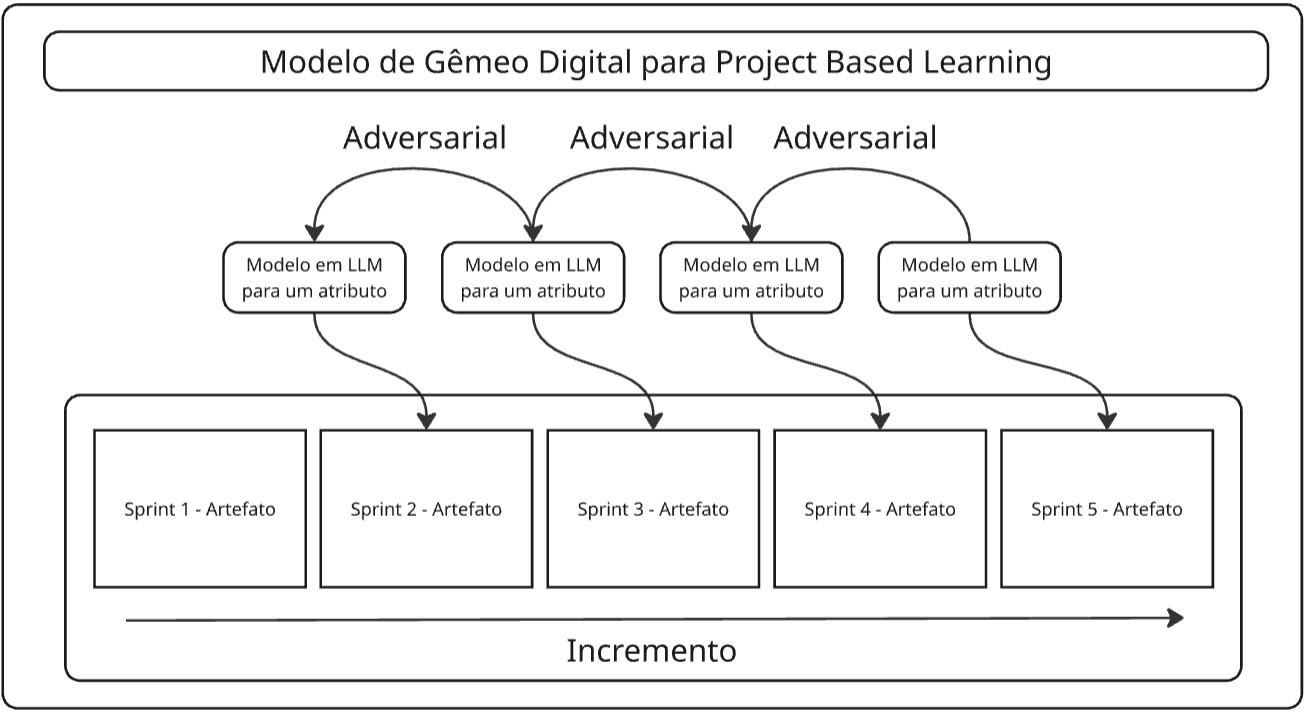
\includegraphics[width=0.8\textwidth]{assets/f1.png}
\caption{Arquitetura Conceitual do Modelo de Gêmeo Digital para Avaliação em PBL}
\label{fig:modelo_proposto}
\end{figure}

A arquitetura apresentada na Figura \ref{fig:modelo_proposto} ilustra como o modelo integra dados provenientes de múltiplas fontes (sistemas de controle de versão, plataformas de colaboração, ferramentas de desenvolvimento, interações presenciais) para construir uma representação virtual abrangente dos processos de aprendizagem. Esta integração permite a captura de métricas quantitativas e qualitativas sobre o progresso dos projetos, a dinâmica das equipes e a assimilação de conceitos pelos estudantes.

\subsection{Componentes do Modelo}

O modelo proposto compreende quatro componentes principais que trabalham de forma integrada para proporcionar avaliação contínua e multidimensional:

\textbf{Camada de Coleta de Dados}: Responsável pela captura de informações em tempo real provenientes das atividades dos estudantes, incluindo dados de repositórios de código, plataformas de comunicação, ferramentas de gestão de projetos e observações diretas. Esta camada implementa conectores específicos para diferentes tipos de fonte de dados, buscando garantir cobertura abrangente das atividades relacionadas aos projetos PBL.

\textbf{Camada de Processamento e Análise}: Aplica algoritmos de análise para transformar os dados brutos em informações significativas sobre o processo de aprendizagem. Inclui módulos específicos para análise das três visões arquiteturais: processamento estrutural (organização de recursos e artefatos), análise comportamental (padrões de colaboração e comunicação) e avaliação processual (aderência a metodologias e cronogramas).

\textbf{Camada de Representação Virtual}: Mantém o modelo digital atualizado do processo de aprendizagem, incluindo representações visuais do progresso dos projetos, mapas de competências desenvolvidas e dashboards de acompanhamento. Esta camada busca garantir a sincronização contínua entre o estado real dos projetos e sua representação virtual.

\textbf{Camada de Interface e Feedback}: Proporciona interfaces adaptadas para diferentes stakeholders (estudantes, docentes, coordenadores), oferecendo visualizações específicas e mecanismos de feedback em tempo real. Inclui alertas automáticos para identificação de dificuldades de aprendizagem e sugestões para intervenções pedagógicas.

\subsection{Visões Arquiteturais Integradas}

Conforme estabelecido pela norma ISO/IEC/IEEE 42010:2022 \cite{iso42010}, o modelo implementa três viewpoints específicos para capturar diferentes aspectos dos processos de aprendizagem:

\textbf{Viewpoint Estrutural}: Mapeia a organização estática dos projetos PBL, incluindo estrutura das equipes, distribuição de recursos, arquitetura dos artefatos produzidos e configuração do ambiente de desenvolvimento. Este viewpoint permite identificação de lacunas organizacionais e inadequações na alocação de recursos que possam impactar o desempenho das equipes.

\textbf{Viewpoint Comportamental}: Modela as interações dinâmicas entre os participantes do processo educacional, capturando padrões de colaboração, frequência e qualidade da comunicação, dinâmicas de resolução de problemas e desenvolvimento de competências transversais. Este viewpoint revela aspectos do processo de aprendizagem que são tradicionalmente difíceis de capturar através de métodos convencionais de avaliação.

\textbf{Viewpoint de Processo}: Representa os fluxos temporais de atividades, marcos de entrega, aderência a metodologias de desenvolvimento de software e evolução qualitativa dos produtos desenvolvidos. Este viewpoint pode oferecer visibilidade sobre a qualidade dos processos adotados pelas equipes e sua conformidade com as melhores práticas da engenharia de software.

\subsection{Considerações de Implementação}

A implementação prática do modelo requer consideração de aspectos técnicos, pedagógicos e éticos específicos do contexto educacional. Do ponto de vista técnico, o sistema deve buscar garantir escalabilidade para suportar múltiplos projetos simultâneos, interoperabilidade com ferramentas existentes no ambiente educacional e performance adequada para análise em tempo real. Do ponto de vista pedagógico, o modelo deve respeitar a natureza construtivista da aprendizagem em PBL, evitando interferências excessivas no processo natural de descoberta e experimentação dos estudantes. Do ponto de vista ético, a implementação deve buscar garantir privacidade dos dados dos estudantes, transparência nos critérios de avaliação e uso responsável das informações coletadas.

\subsubsection{Abordagem Metodológica: Case de Estudo e Escolha Tecnológica}

Em conformidade com os princípios de design centrado no usuário e arquitetura orientada a requisitos, a validação do modelo proposto será conduzida através de um \textbf{case de estudo} específico que permitirá implementação prática e avaliação empírica da eficácia do gêmeo digital de processos e sistemas em contexto real de PBL.

O case de estudo seguirá a filosofia de que \textbf{a tecnologia representa sempre a última camada a ser definida} no processo de design, priorizando a compreensão profunda dos requisitos pedagógicos, necessidades dos usuários (estudantes e docentes) e objetivos educacionais antes da seleção de ferramentas e plataformas tecnológicas específicas. Esta abordagem busca garantir que as soluções tecnológicas sejam escolhidas com base em critérios de adequação funcional e pedagógica, não por limitações ou preferências tecnológicas pré-concebidas.

A estrutura do case de estudo contemplará:

\textbf{Definição do Contexto}: Seleção de uma disciplina de engenharia de software que utilize metodologia PBL, preferencialmente em nível de graduação ou pós-graduação, com projetos de complexidade adequada para demonstração das capacidades do gêmeo digital de processos e sistemas.

\textbf{Identificação de Stakeholders}: Mapeamento dos parceiros educacionais (análogo aos business drivers do modelo Inteli), incluindo docentes orientadores, estudantes participantes, coordenação acadêmica e, quando aplicável, parceiros externos que fornecem desafios autênticos para os projetos.

\textbf{Especificação de Requisitos}: Definição detalhada dos requisitos funcionais e não funcionais do sistema, considerando as três visões arquiteturais (estrutural, comportamental e de processo) e as necessidades específicas do contexto educacional escolhido.

\textbf{Seleção Tecnológica Criteriosa}: Somente após a completa especificação de requisitos, será realizada a seleção de tecnologias, ferramentas e plataformas que melhor atendam aos objetivos pedagógicos identificados. Esta seleção considerará critérios como facilidade de integração com ambientes educacionais existentes, capacidade de coleta de dados em tempo real, escalabilidade, usabilidade para docentes e estudantes, e custos de implementação e manutenção.

\textbf{Implementação Iterativa}: O desenvolvimento do gêmeo digital seguirá metodologias ágeis de desenvolvimento de software, permitindo refinamentos contínuos baseados em feedback dos usuários e análise dos resultados parciais obtidos durante o case de estudo.

Esta abordagem metodológica busca assegurar que o foco do doutorado permaneça na \textbf{criação do modelo conceitual de gêmeo digital de processos e sistemas} para avaliação educacional, utilizando o case de estudo como meio de validação prática sem que a escolha de tecnologias específicas limite ou comprometa a generalidade e aplicabilidade do modelo proposto.

\section{METODOLOGIA}

Em criação...

\section{CRONOGRAMA}

O desenvolvimento desta pesquisa de doutorado está estruturado em fases sequenciais e sobrepostas, distribuídas ao longo de um período de 9 meses, culminando com a qualificação prevista para março de 2026. O cronograma apresentado na Tabela \ref{tab:cronograma} detalha as principais atividades e seus respectivos períodos de execução.

\begin{table}[htbp]
\centering
\caption{Cronograma de Execução da Pesquisa}
\label{tab:cronograma}
\small
\begin{tabular}{|l|c|c|c|c|c|c|c|c|c|}
\hline
\textbf{Atividade} & \textbf{Jul} & \textbf{Ago} & \textbf{Set} & \textbf{Out} & \textbf{Nov} & \textbf{Dez} & \textbf{Jan} & \textbf{Fev} & \textbf{Mar} \\
\hline
Pesquisa Bibliográfica & X & X & X & & & & & & \\
\hline
Proposição do Modelo & & X & X & & & & & & \\
\hline
Case de Estudo & & & & X & X & X & & & \\
\hline
Análise de Resultados & & & & & & X & X & X & \\
\hline
Preparação Qualificação & & & & & & & & X & X \\
\hline
\textbf{Qualificação} & & & & & & & & & \textbf{X} \\
\hline
\end{tabular}
\end{table}

\textbf{Fase 1 - Pesquisa Bibliográfica (Julho-Setembro 2025)}: Revisão sistemática da literatura sobre gêmeos digitais aplicados à educação, metodologias PBL em engenharia de software, e frameworks de avaliação educacional. Esta fase incluirá a análise crítica de trabalhos correlatos e a identificação de lacunas de pesquisa que justifiquem a originalidade da proposta.

\textbf{Fase 2 - Proposição do Modelo (Agosto-Setembro 2025)}: Desenvolvimento do modelo conceitual de gêmeo digital de processos e sistemas para avaliação de projetos PBL, incluindo a especificação detalhada das três visões arquiteturais (estrutural, comportamental e de processo), definição de métricas e indicadores de avaliação, e elaboração dos requisitos funcionais e não funcionais do sistema.

\textbf{Fase 3 - Case de Estudo (Outubro-Dezembro 2025)}: Implementação prática do modelo proposto em contexto real de PBL, incluindo seleção do ambiente educacional, especificação de requisitos específicos do contexto, escolha criteriosa de tecnologias adequadas, desenvolvimento do protótipo funcional, e coleta de dados empíricos para validação.

\textbf{Fase 4 - Análise de Resultados (Dezembro 2025 - Fevereiro 2026)}: Processamento e análise dos dados coletados durante o case de estudo, validação das hipóteses de pesquisa através de testes estatísticos apropriados, avaliação da eficácia do modelo proposto, e documentação dos resultados obtidos.

\textbf{Fase 5 - Preparação para Qualificação (Fevereiro-Março 2026)}: Consolidação de todos os resultados em documento de qualificação, preparação da apresentação oral, e ajustes finais baseados em revisões do orientador e colaboradores.

A \textbf{Qualificação} está prevista para \textbf{março de 2026}, quando serão apresentados todos os resultados obtidos nas fases anteriores, incluindo o modelo conceitual validado, os resultados empíricos do case de estudo, e as contribuições científicas da pesquisa para as áreas de educação em engenharia e tecnologias educacionais emergentes.

\def\refname{REFERÊNCIAS BIBLIOGRÁFICAS}
\bibliography{biblproj}
\addcontentsline{toc}{section}{REFERÊNCIAS BIBLIOGRÁFICAS}
\bibliographystyle{abnt-alf}

\end{document}
